\documentclass{article}
\usepackage[utf8]{inputenc}
\usepackage[margin=0.2in]{geometry}
\usepackage{graphicx}
\graphicspath{ {./images/} }
\usepackage{graphicx,wrapfig,lipsum}

\begin{document}
\twocolumn
{\huge Elektriahelad: RC-vooluringid}\\
{\Large Saskia, nr4 2021}\\
\section{Takistid ja lambid}
\subsection{Lampide eredus}
Pingeallikaga on rööbiti ühendatud kaks lampi, kusjuures üks lampidest põleb
k korda suurema võimsusega kui teine. Seejärel ühendatakse need lambid sama
pingeallikaga jadamisi. Kuidas muutub lampide ereduste summa? Vihje: Lampide eredus sõltub võimsusest.
\subsection{12 Lampi}
Juku käsutuses on 12 ühesugust taskulambipirni ning patarei, mille klemmipinge on täpselt 5 korda suurem pirni nimipingest. Lisaks leidis ta juhtumisi takisti,
mille takistus on parajasti pool lambi hõõgniidi takistusest töörežiimis (viimase
sai ta teada jagades lambi soklile kirjutatud nimipinge ja -voolu omavahel).\\
a) Kuidas tuleb ühendada nimetatud komponendid elektriahelasse, et kõik 12 pirni põleksid normaalheledusega?\\
b) Mitu korda kasvab (või kahaneb) lampide koguvõimsus, kui üks lampidest läbi
põleb?
\subsection*{Kirchhoff jms}
Elektriahelas tekitab voolu elektromotoorjõud $\varepsilon$. See on patarei pinge, kus on arvesse võetud ka patarei enda takistus ehk sisetakistus r. $U = \varepsilon - Ir$\\
\textbf{Kirchhoffi I seadus} e vooluseadus: 
Voolutugevuste algebraline summa juhtmete sõlmpunktis on 0.  $\sum I = 0$\\
Praktiline järeldus on, et elektriahela sõlme suunduvate harude voolutugevuste summa on võrdne väljuvate harude voolutugevuste summaga. $I_{in} = I_{out}$\\
\textbf{Kirchhoffi II seadus} e pingeseadus: Kinnise kontuuri pingelangude algebraline summa $\sum U = 0$. \\
Kasutuskõlblikum versioon sellest on, et kinnise kontuuri elektromotoorjõudude summa on võrdne takistitel tekkivate pingelangude summaga. $\sum \varepsilon = \sum U_R$\\
Harjutamiseks leia takistus klemmide vahel:\\
a)\\
\begin{center}
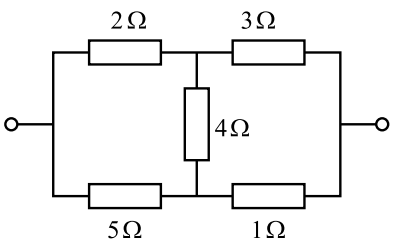
\includegraphics[width =  7cm]{ec3.PNG}
\end{center}
b)\\
\begin{center}
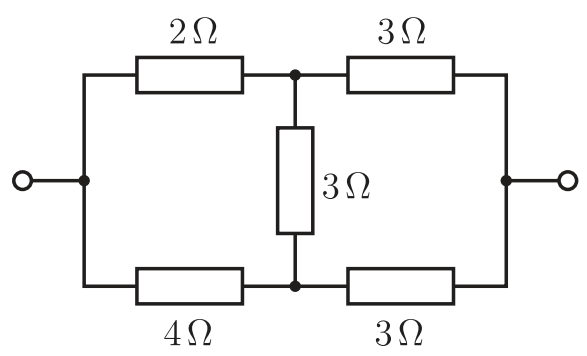
\includegraphics[width =  7cm]{ec4.PNG}
\end{center}
\subsection{Kirchhoffi labürint}
Kõigi takistite $R=4\Omega$. Kõik patareid on ideaalsed ning elektromotoorjõud $\varepsilon = 4V$. Leia vool läbi takisti R.
\begin{center}
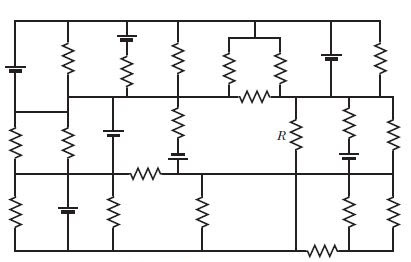
\includegraphics[width =  7cm]{ec2.jpg}
\end{center}
\subsection{Piirkond 2013 G5}
Joonisel toodud skeemil on ampermeetrid ideaalsed; patareide elektromotoorjõud ja sisetakistused on märgitud nende juurde. Leidke ampermeetrite näidud, kui\\
a) lüliti on suletud\\
b) lüliti on lahti.
\begin{center}
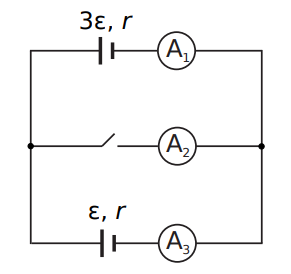
\includegraphics[width =  3cm]{ec12.PNG}
\end{center}
\subsection{IPhO 1996}
Leia takistus punkti A ja B vahel
\begin{center}
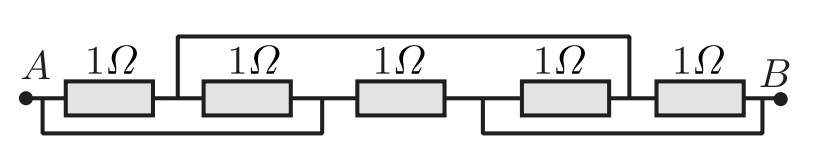
\includegraphics[width =  7cm]{ec5.PNG}
\end{center}
\subsection{Kuup}
Kuubi iga külje takistus on 1$\Omega$. Leia klemmidevaheline takistus.
\begin{center}
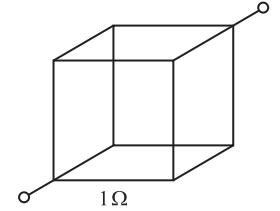
\includegraphics[width =  3cm]{ec10.PNG}
\end{center}
\subsection{Kaheksanurk}
Kaheksanurga kõik diagonaalid on traadijupid takistusega R. Kaheksanurga küljed on insuleerivad. Paku, mis vahemikus võib olla kahe lähisnurga vaheline takistus.
\subsection{Kuusnurk}
Kuusnuga ABCDEF iga nurk on ühendatud kuusnurga keskpunktiga O kasutades takistusega R traadijuppe. Ka igal kuusnurga külg on takistusega R. Leia takistus A ja O vahel.
\subsection{Võre}
Leia punktide A ja B vaheline takistus. Ruudustiku naaberpunktid on ühendatud 1-oomilise traadijupiga.
\begin{center}
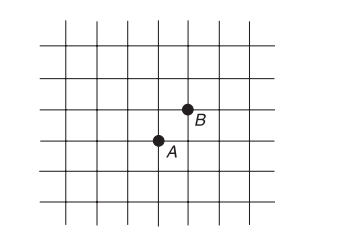
\includegraphics[width =  3cm]{ec11.png}
\end{center}
\subsection{}
Mis on eelnevas ülesanded takistus, kui A ja B vaheline traadijupp läbi lõigatakse?
\subsection{Lõpmatu ahel}
Leia antud lõpmatu, kuid perioodilise ahela takistus.
\begin{center}
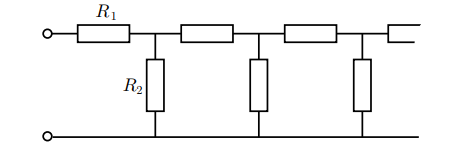
\includegraphics[width =  7cm]{ec14.PNG}
\end{center}
\section{Kondensaatorid}
\begin{center}
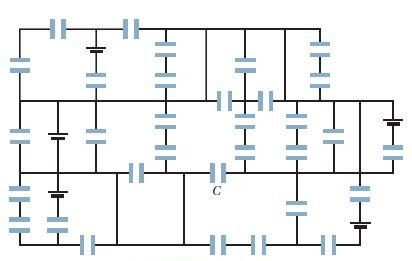
\includegraphics[width =  7cm]{ec1.jpg}
\end{center}
\begin{center}
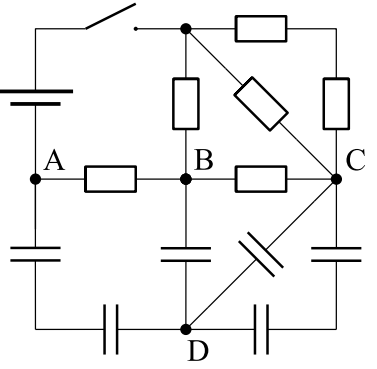
\includegraphics[width =  7cm]{ec6.PNG}
\end{center}
Juuresoleval skeemil on alguses lüliti avatud. Leidke takistitel
eralduv koguvõimsus
(a) vahetult pärast lüliti sulgemist;
(b) pika aja möödudes pärast lüliti sulgemist.
Kõikide takistite takistus on R ja patarei pinge on V . 
\begin{center}
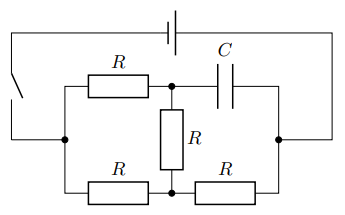
\includegraphics[width =  3cm]{cap1.PNG}
\end{center}

An hexagon ABCDEF with six “spokes” (connecting its centre O with the vertices) is made of 12 pieces of
wire, each having a electrical resistance R. Find the resistance
between the vertices A and O using methods 20 and 21.\\
There is an octagon all diagonals of which are resistors of equal resistance R; the sides of the octagon are made
of an insulating material. Find lower and upper bounds for the
resistance between two neighbouring nodes of such an octagon.
Leidke juuresoleval skeemil voolutugevus I läbi ampermeetri kahel juhul: vahetult pärast lüliti sulgemist ja pika aja möödumisel. Eeldada, et kondensaatorid on
enne lüliti sulgemist laadimata. Patarei lugeda ideaalseks.\\
\begin{center}
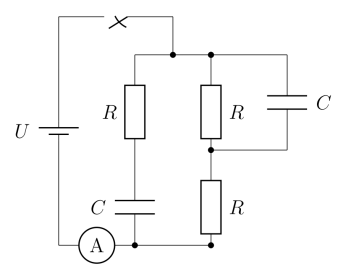
\includegraphics[width =  3cm]{cap2.PNG}
\end{center}
\section{Muutlikud vooluahelad}
\subsection{Dioodid}
pr 29. [EstOPhC-2012]
\end{document}